\chapter{Metodologia}\label{chap:metodologia}

[TO DO]

\section{Descrição do Problema}

\subsection{Aprendizado Profundo (Deep Learning)}
O Aprendizado Profundo é um campo especializado de aprendizado de máquina, onde sua principal característica e diferenciação de outros campos de aprendizado de máquina é o uso de redes neurais artificiais com múltiplas camadas, assim é possível aprender e extrair informações complexas por meio de um grande volume de dados.

\subsection{Redes Neurais Artificiais}
A rede neural artificial é um modelo computacional baseado na estrutura de um cérebro humano, pois tenta imitar a forma de como os neurônios se conectam e processam sinais eletroquímicos em nosso cérebro para aprender a partir de dados,
identificando padrões e tomando decisões. Todo esse processo ocorre através do perceptron multicamadas (MLP), que é um modelo de deep learning que possui funções matemáticas que mapeiam um conjunto de valores de entrada para valores de saída.
Em uma rede neural, por exemplo, milhões de imagens de um objeto são processadas para que a rede possa aprender, através de características visuais que definem aquele objeto para assim ser reconhecido posteriormente.

Uma rede neural profunda é composta por unidades (nós) interconectadas, organizadas em camadas.

\begin{itemize}
    \item \textbf{Nó (neurônio):} É uma unidade computacional em que armazena e calcula uma soma ponderada das entradas mais um bias e passa o resultado através de uma função de ativação, produzindo uma saída.
    \item \textbf{Camada de Entrada (Input Layer):} É onde todo o processo é iniciado, é nela que os dados são introduzidos na rede. O número de nós nessa camada é o número de características dos dados de entrada.
    \item \textbf{Camadas Ocultas (Hidden Layers):} São camadas intermediárias entre a entrada e a saída, cada nó em uma camada oculta está conectado a todos os nós da camada anterior e da camada seguinte. Nas camadas ocultas é onde ocorre a maior parte de todo processamento e aprendizado, a saída de uma camada oculta é utilizada como entrada para a próxima, a cada camada oculta, a rede aprende a detectar características mais complexas e abstratas a respeito dos dados de entrada. Camadas iniciais ocultas aprendem características simples, em que cada camada seguinte utiliza as informações da camada anterior para aprender características mais complexas. Redes com múltiplas camadas ocultas são as chamadas \textit{Deep Learning}.
    \item \textbf{Camada de Saída (Output Layer):} Camada final da rede, é nela que o resultado final é produzido. A estrutura da camada de saída depende da tarefa, podendo ser de regressão, que prevê um valor contínuo, possuindo um nó com uma função de ativação linear, pode ser de classificação binária, com um único neurônio que expressa resultados binários, sim ou não. Há também a classificação multiclasse, que possui um nó para cada classe possível, e a saída com maior valor de ativação é o resultado final.
\end{itemize}

Para a conexão entre os nós e as camadas, há arestas que ligam uns aos outros. Cada conexão tem um peso associado, esse peso é o que determina a importância daquela conexão.
Um peso alto significa que aquela conexão é muito importante para o próximo neurônio, já um peso próximo a zero, demonstra que terá pouco ou nenhuma influência.
Cada nó de uma camada está conectada a todos os nós da próxima camada, cada uma dessas conexões possuem seus próprios pesos com valores aleatórios iniciais, que serão ajustados durante o treinamento.

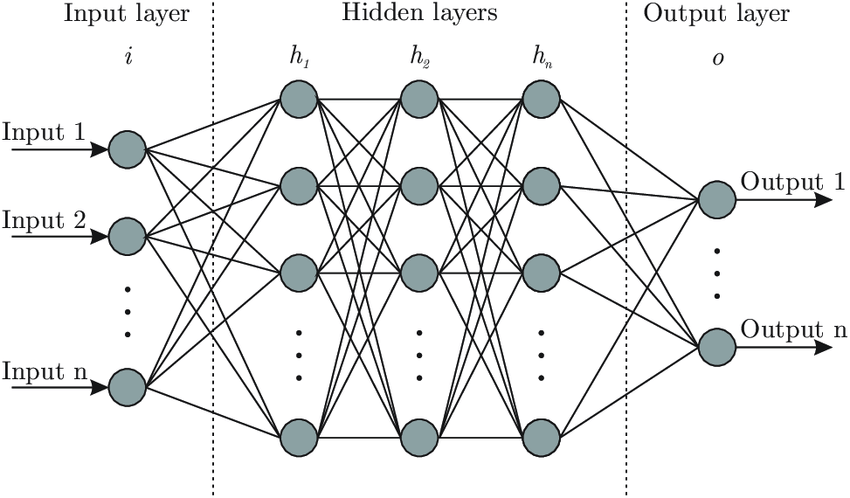
\includegraphics[scale=0.45]{03_capitulo/imageArquiteturaRedeNeural.png}

\subsection{Bias em Redes Neurais}
Bias são parâmetros adicionais que ajustam a saída de um neurônio, sendo valores numéricos associados a cada neurônio, não estando ligado a nenhuma entrada específica, atua como um coeficiente linear.
Há uma soma ponderada das entradas de um neurônio e adiciona o bias, um valor constante, antes que o resultado seja passado para a função de ativação.
A principal função do bias é deslocar a função de ativação para que o modelo possa se ajustar melhor aos dados, sem o bias, a soma ponderada teria que ser alta para que o neurônio ativasse, com o bias, mesmo que a soma ponderada seja baixa, o neurônio pode ativar se o bias for alto. Logo, um bias alto torna fácil o neurônio ser ativado, precisa de menos estímulos dos pesos, já um bias negativo alto, dificulta a ativação do neurônio, precisa de mais estímulos dos pesos. Sem a existência de um bias, um nó só se ativaria quando a entrada atingisse um limite específico.
O bias é um parâmetro aprendível, assim, o próprio modelo descobre quais são os melhores valores durante o treinamento. Inicialmente eles são inicializados como zero ou valores muito baixos, e durante o treinamento o backpropagation calcula o gradiente da função de erro também para cada bias, indicando quanto aquele bias contribui para o erro total. Por meio de um otimizador, como o gradiente descendente, o bias é atualizado para minimizar o erro. A cada iteração o bias é ajustado, fazendo com que o modelo se adapte melhor aos dados.

\subsection{Função de Ativação}
A função de ativação é como um filtro, em que determina a saída do neurônio com base na entrada recebida, sendo uma função matemática aplicada a cada nó da rede neural, em que atua na soma ponderada das entradas de um neurônio após a adição do bias.
Com a função de ativação, o modelo pode aprender e representar padrões complexos nos dados, introduzindo não linearidade no modelo, em que permite que ao combinar multicamadas, aprenda e represente relações complexas e curvas, conseguindo resolver problemas complexos que não podem ser resolvidos com uma simples função linear, pois com a linearidade, cada nó estaria realizando uma transformação linear, assim uma sequência de nós resultaria em uma única transformação linear, seria como o modelo tivesse uma única camada.

A ativação de um nó ocorre em 3 etapas:
\begin{itemize}
    \item O nó pega o valor de ativação da camada anterior e multiplica pelo peso que une ele ao nó, faz isso com todos os nós que chegam até ele e por fim, soma tudo. O peso atua para controlar a importância, no qual um alto peso amplifica o sinal de entrada, um baixo ou negativo, diminui.
    \item Após a soma ponderada, o Bias é adicionado, é um valor que funciona como um auxílio, seja positivo ou negativo, para que o neurônio ative, define quão alta a soma ponderada precisa ser para o neurônio ativar.
    \item O resultado (soma ponderada + bias) é passado por uma função de ativação, função que produz a saída final do neurônio. Esse resultado é então passado para os nós da próxima camada.
\end{itemize}
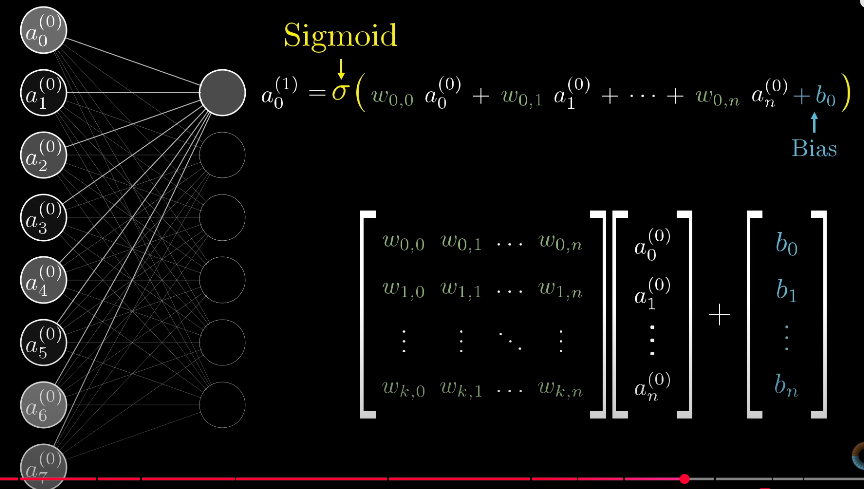
\includegraphics[scale=0.55]{03_capitulo/imageMatrizes_sigmoid.png}

Há diversas funções de ativação, cada uma com suas próprias características e aplicações.
\begin{itemize}
    \item \textbf{ReLU (Rectified Linear Unit):} Função de ativação mais utilizada em redes neurais, em que é uma linha reta com inclinação 1 para valores positivos e 0 para negativos, sendo computacionalmente muito eficiente e não havendo desaparecimento do gradiente, pois a inclinação é constante para entradas positivas e como os neurônios com entradas negativas são desativadas, a rede se torna esparsa e eficiente. Porém, pode sofrer com o problema de Dying ReLU, neurônio morto, em que se um neurônio recebe várias entradas negativas durante o treinamento, seu peso fica ajustado em que sua entrada seja sempre negativa, assim ele nunca mais será reativado, parando de aprender.
    \item \textbf{Sigmoid:} Função que mapeia qualquer valor real para um valor entre 0 e 1, sendo útil para problemas de classificação binária, já que uma saída entre 0 e 1 pode ser interpretada como uma probabilidade. Caiu em desuso pois quando há entradas muito altas ou muito baixas, a inclinação da curva é quase zero, assim o gradiente fica muito pequeno, fazendo com que o aprendizado seja muito lento ou até pare.
    \item \textbf{Tanh (Tangente Hiperbólica):} É uma melhoria referente a Sigmoid, mapeia qualquer valor real para um valor entre -1 e 1, assim é centrada em zero, o que pode ajudar na convergência do modelo. Porém, assim como a Sigmoid, sofre com o problema do gradiente desaparecendo.
    \item \textbf{Softmax:} A função Softmax difere das outras, pois ela não é usada em neurônios individuais nas camadas ocultas, mas sim aplicada a todos os neurônios na camada de saída, em que um vetor de números reais, saídas brutas da última camada, é transformado em um vetor de probabilidade, onde cada valor está entre 0 e 1. Acaba sendo utilizada para problemas de classificação multiclasse, onde cada nó na camada de saída representa uma classe diferente, e a saída do Softmax indica a probabilidade de cada classe.
\end{itemize}

Ativações em uma camada determinam ativações na camada seguinte.
De acordo com o que é inserido, que causa ativação, causa um padrão de ativação específico na camada seguinte, que vai à seguinte e assim sucessivamente até produzir o resultado final. De camada em camada as ativações vão criando um padrão cada vez mais complexo e abstrato.
Cada camada aprende a reconhecer padrões cada vez mais sofisticados baseados nos padrões da camada anterior.

Se o modelo busca identificar números escritos a mão, na camada de saída, cada nó representará um número de 0 a 9, e o nó que tiver a maior ativação será o número identificado.

\subsection{Compressão de Modelos}
Com o crescimento da \textit{Deep Learning}, os modelos de \textit{IA} cresceram em tamanho ao longo dos anos, dobrando a cada 2,4 anos,
uma vez que os modelos de redes neurais atuais de alta performance são treinados para serem os mais precisos possível, sendo modelos matemáticos com uma grande quantidade de parâmetros que ocupam muito armazenamento,
sendo principalmente um problema para dispositivos com capacidade limitada de armazenamento e processamento, onde a execução desses modelos necessitam de um grande número de operações de pontos flutuantes (FLOPS), sendo assim necessitam de muito tempo para processar todas as entradas e obter uma resposta.

Portanto, a compressão de modelos é um campo de estudo e conjunto de técnicas que tentam amenizar esses problemas de complexidade computacional, minimizando seu tamanho e/ou quantidade de cálculos com o intuito de manter uma acurácia satisfatória.
As redes neurais possuem uma alta redundância de parâmetros, assim a compressão de modelos tem como objetivo remover pesos que possuem baixa contribuição ao resultado final.
Há 4 principais formas de compressão.
\begin{itemize}
    \item \textbf{Quantização (Quantization):} Técnica de compressão de modelo que reduz o número de bits para representar cada peso no modelo, ao invés dos parâmetros serem armazenados em pontos flutuantes de 32bits, a quantização mapeia esses valores e passa para uma menor precisão, como 16bits ou até 8bits, assim o modelo já reduz automaticamente e as operações com números inteiros, por exemplo, são mais simples do que com pontos flutuantes.
    \item \textbf{Destilação de Conhecimento (Knowledge Distillation):} Metodologia de treinamento, no qual utiliza de um modelo grande de alta performance já treinado, um modelo "professor" e então há um modelo de arquitetura menor e mais eficiente, o "aluno". Durante o treinamento, o modelo "aluno" aprende a minimizar uma função de custo, que uma parte tenta acertar rótulos verdadeiros dos dados e outras tenta imitar a distribuição de probabilidade de saída do modelo "professor", assim tem-se um modelo "aluno" compacto que alcança uma precisão maior do que se tivesse sido treinada do zero.
    \item \textbf{Fatoração de Matrizes (Matrix Factorization):} Matrizes de pesos de uma camada que pode ser muito grande é decomposta em duas ou mais matrizes menores, e o resultado dessas matrizes menores se aproxima da matriz original durante a inferência, que assim exigem um menor custo computacional que a matriz original.
    \item \textbf{Poda Neural (Neural Pruning):} A poda é o processo de remoção de pesos ou até nós inteiros que não impactam ou impactam pouco para o resultado final do modelo. A poda será detalhada na Seção \ref{sec:pruning}.
    %figura do artigo Learning both Weights and Connections for Efficient Neural Networks
    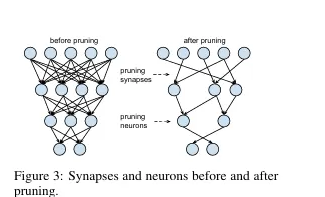
\includegraphics{03_capitulo/imagepoda.png}
\end{itemize}

\subsection{Consumo de energia}
Com o avanço de técnicas e de hardware para o treinamento de redes neurais, com o intuito de atingir resultados mais eficientes, demanda um consumo de energia considerável,
assim, uma grande emissão de carbono na atmosfera, sendo que o treinamento de um modelo de um transformer com busca de arquitetura neural emite cerca de 626.155 lbs de CO2, enquanto um carro ao longo de toda a sua vida útil emite cerca de 126.000 lbs, cerca de 4.9 vezes menos.
Todo esse consumo de energia se deve a duas etapas do ciclo de um modelo, o treinamento e a inferência.

No processo de treinamento, o modelo é alimentado com um grande volume de dados que são ajustados em um processo de tentativa e erro (back propagation), requerem hardwares especializados com GPUs ou TPUs, organizados em clusters com centenas ou milhares de processadores.

No processo de inferência, que é o processo de utilizar esse modelo já treinado para fazer requisições e obter respostas, uma resposta que o modelo dá, gasta pouca energia, mas olhando para um contexto de larga escala de uso em que as IAs generativas estão inseridas, o custo energético total é significativo.

\section{Treinamento de Redes Neurais}

\subsection{Gradiente}
Quando se fala de gradiente em redes neurais, está se referindo ao vetor de derivadas parciais da função de perda em relação aos pesos da rede neural, é ele que permite a minimização da função de perda através do algoritmo de descida do gradiente, em que é um método de primeira ordem que utiliza informações do gradiente para atualizar os parâmetros da rede.
O gradiente é um vetor de derivadas para uma função que recebe um vetor de variáveis de entrada, cada componente no vetor de gradiente é uma derivada parcial, em que é calculada assumindo que todas as outras variáveis da função são mantidas constantes, assim o gradiente é capaz de capturar a inclinação da função e assim permite prever o efeito da alteração.

Gradiente está extremamente ligado à derivada, que é uma taxa de mudança de uma função em um ponto específico, ou seja, a derivada informa a linha tangente em um ponto, e essa inclinação pode ser usada para estimar o valor da função em um próximo ponto, em que o valor da derivada indica quanto a função está mudando, sua magnitude, e a direção, o sinal. Se a derivada é positiva, a função está aumentando, se é negativa, a função está diminuindo.

\subsection{Backpropagation}
É um algoritmo utilizado para que as redes neurais aprendam, pois é ele que possibilita que a rede ajuste seus parâmetros internos (pesos e bias) com o intuito de calcular a contribuição de cada parâmetro da rede para o erro final de previsão, melhorando a performance do modelo.
Ao fim do treinamento, com o erro já calculado, o algoritmo de backpropagation faz um fluxo invertido do treinamento, indo da camada de saída até a camada de entrada, em que o erro calculado na camada de saída é propagado para as camadas anteriores da rede, assim os pesos e bias são ajustados para que na próxima iteração o erro seja menor.
O algoritmo de backpropagation é capaz de saber como cada peso individual se correlaciona com o erro, por meio de calcular a derivada parcial do erro em relação a cada peso, para isso o algoritmo usa a regra da cadeia multivariada, em que decompõe o cálculo da derivada em derivadas intermediárias. Após as derivadas parciais calculadas para todos os pesos, esses valores são usados para otimizar a rede, ajustando o peso na direção oposta ao gradiente: se o sinal da derivada de um peso for positivo, logo o peso deve ser diminuído para minimizar o erro, pois assim há uma menor função de perda.
A atualização dos parâmetros é feita pelo algoritmo de otimização (gradiente descendente), sendo: parâmetroNovo = parâmetroAntigo - (taxa de aprendizado * gradiente do parâmetro). Dessa forma corrige os parâmetros na direção oposta ao gradiente, reduzindo a função de perda. O que controla o tamanho desse ajuste é o hiperparâmetro da taxa de aprendizado.

\subsection{Hiperparâmetros}
Hiperparâmetros são variáveis externas que definem tanto o algoritmo de aprendizado quanto a arquitetura da rede neural. Ao contrário dos parâmetros do modelo (pesos e biases) que são ajustados pelo backpropagation, os hiperparâmetros são definidos antes do início do treinamento, são eles que controlam como a rede neural aprende, ditam como o modelo irá aprender a partir dos dados, esses hiperparâmetros são dados por terceiros, em que vão testando os valores até chegar em um resultado satisfatório. Há técnicas de automatização de busca para encontrar boas combinações de hiperparâmetros, como busca em grade ou otimização bayesiana, mas o ajuste manual baseado na experiência ainda é frequentemente preferido e pode acabar produzindo um melhor desempenho.
Há duas principais categorias de hiperparâmetros.
\begin{itemize}
    \item \textbf{Hiperparâmetros de arquitetura da rede:} Definem a estrutura interna da rede antes mesmo de qualquer inserção de dados, seja ela o número de camadas ocultas, o número de neurônios em cada camada e o tipo de função de ativação utilizada.
    \item \textbf{Hiperparâmetros do processo de treinamento:} Controlam como o modelo se ajusta aos dados durante o treinamento, seja a taxa de aprendizado, em que controla o tamanho do passo em que o algoritmo de otimização dá ao ajustar os pesos na rede, número de épocas, que é o número de vezes que o algoritmo de treinamento irá passar por todo o conjunto de dados de treinamento, tamanho do lote, que são o número de exemplos de treinamento utilizados em uma única iteração, para calcular o erro e atualizar os pesos, e o algoritmo de otimização, sendo a escolha do algoritmo para aplicar os gradientes calculados pelo Backpropagation.
\end{itemize}

\subsection{Passo a passo do treinamento de uma rede neural}
Para um treinamento de uma rede neural do zero é necessário um grande conjunto de dados rotulados, ou seja, cada dado de entrada deve ter uma saída correta associada, para que o modelo possa aprender a partir desses exemplos.
O conjunto deve ser dividido em três partes: conjunto de treinamento, conjunto de validação e conjunto de teste. O conjunto de treinamento é usado para ajustar os pesos e bias da rede, o conjunto de validação é usado para monitorar o desempenho do modelo durante o treinamento e ajustar hiperparâmetros, e o conjunto de teste é usado para avaliar de forma imparcial o desempenho final do modelo após o treinamento.
Tendo também de haver uma definição da arquitetura da rede neural, sendo a quantidade de camadas, quantidade de nós em cada camada, função de ativação, podendo haver diferentes funções de ativação em diferentes camadas e definição dos hiperparâmetros, como taxa de aprendizado, tamanho do lote (batch size) e o número de épocas.
Todo o treinamento de uma rede neural ocorre em um grande número de iterações, em que cada passagem completa pela rede é chamada de época (epoch) e em cada época, os dados são processados em pequenos lotes (batches).

Os nós da primeira camada recebem os dados que serão treinados, seguindo um exemplo de uma rede neural que identifica objetos, essa imagem sendo 28px x 28px, terá 784 nós na camada de entrada, onde cada nó receberá um valor do pixel da imagem, valor esse referente a intensidade do pixel, a uma característica do dado que está sendo analisado.

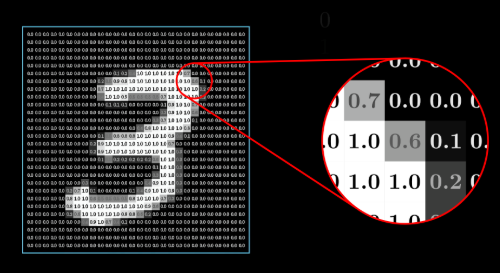
\includegraphics[scale=0.8]{03_capitulo/pixel-nos.png}

\begin{itemize}
    \item \textbf{Passo 1 (Inicialização dos Parâmetros):} Antes de qualquer iteração, os pesos e bias da rede são inicializados com valores baixos e aleatórios, em que o bias são inicializados com zero. Dessa forma, qualquer simetria que possa ser gerada é quebrada, permite que cada nó aprenda pontos diferentes, pois se eles fossem inicializados com o mesmo valor, todos os neurônios aprenderiam as mesmas características dos dados.
    \item \textbf{Passo 2 (Forward Pass):} Um lote dos dados de treinamento é inserido na camada de entrada, passando por todas as camadas ocultas, onde cada nó realiza a soma ponderada das entradas mais o bias e o resultado passa para a função de ativação, assim, a saída de uma camada se torna a entrada da próxima camada, até chegar na camada de saída, em que produz uma previsão.
    \item \textbf{Passo 3 (Loss Calculation):} Nessa etapa a previsão da rede emitida pela camada de saída é comparada com a saída correta, os rótulos verdadeiros, e então é calculada a função de perda, em que quantifica o erro da previsão da rede, dessa forma obtém-se um valor numérico que indica o quão longe a previsão está do valor real.
    \item \textbf{Passo 4 (Backpropagation):} Com o erro calculado, o algoritmo de backpropagation é executado, propagando o erro de volta através da rede, da camada de saída até a camada de entrada, calculando o gradiente da função de perda em relação a cada peso e bias, indicando a direção e a magnitude do ajuste necessário, conforme descrito na seção anterior.
    \item \textbf{Passo 5 (Atualização dos Parâmetros):} Com os gradientes calculados, o algoritmo de otimização atualiza todos os pesos e bias na direção oposta ao gradiente, reduzindo a função de perda.
    \item \textbf{Passo 6 (Repetição):} Os passos 2 a 5 são repetidos para cada lote de dados no conjunto de treinamento, e esse processo é repetido por um número definido de épocas, ou seja, o modelo passa por todo o conjunto de treinamento várias vezes, ajustando os pesos e bias a cada iteração.
\end{itemize}
Todo o ciclo é repetido pelo número de épocas definido, o treinamento é interrompido se o modelo atingir uma precisão satisfatória ou se a função de perda não estiver mais diminuindo significativamente.

\section{Poda Neural (Pruning)}\label{sec:pruning}
A poda é uma técnica de compressão de modelos que tem como objetivo reduzir o tamanho do modelo e o custo computacional, removendo pesos que impactam pouco para o resultado final do modelo.
Todo o processo de poda ocorre após o treinamento inicial do modelo, onde o foco é apenas na performance, assim o modelo atinge a maior acurácia possível, sem pensar em nenhum custo.

\subsection{Tipos de Poda}
Há dois tipos de poda neural:
\begin{itemize}
    \item \textbf{Poda não estruturada:} Remoção de pesos individuais, independente da sua posição na matriz de pesos, seja em qualquer camada da rede, dessa forma oferece maior flexibilidade e geralmente maior taxa de compressão com uma menor perda de acurácia, entretanto requer um hardware mais especializado para que a poda ocorra de forma mais rápida, pois processadores por padrão não são eficientes em pular operações com zeros espalhados de forma aleatória.
    \item \textbf{Poda estruturada:} Remoção de neurônios, filtros ou canais inteiros, o que remove por completo um detector de características, isso já faz com que tenha um grande ganho de velocidade de processamento com hardwares padrões, criando matrizes menores, mas ainda densas, ficando mais fácil de ocorrer a multiplicação no hardware. Entretanto, por remover uma estrutura por completo, a perda de acurácia tende a ser maior.
\end{itemize}

\textbf{Esparsidade Estruturada}: Impõe uma regra mais organizada, não remove pesos aleatoriamente, o algoritmo de poda é forçado a cada pequeno bloco de 4 pesos, 2 deles devem ser zerados. Assim, como o hardware sabe que sempre haverá apenas 2 valores a cada bloco de 4, ele comprime a matriz pela metade, para saber onde estavam os valores não nulos, ele armazena pequenos índices.

Através da poda estruturada o número de operações matemáticas durante a inferência é diretamente reduzido, com isso, a resposta tende a ficar mais rápida e com menor consumo de energia.

\subsection{Poda por Magnitude}
A técnica mais simples e intuitiva de poda é a poda por magnitude, em que os pesos que possuem os valores absolutos mais próximos a zero, após o treinamento inicial, são considerados pouco influentes no resultado final. É definido um limite de poda, onde se decide podar qualquer peso cuja magnitude seja menor que um limiar, por exemplo 0.1, pois ao final, a contribuição deles para o cálculo final será muito baixa, criando redes esparsas.
%figura do artigo
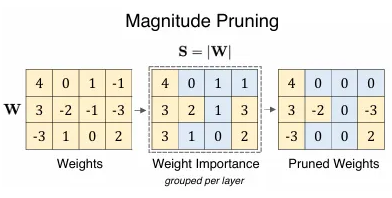
\includegraphics{03_capitulo/imagepodamagnitude.png}

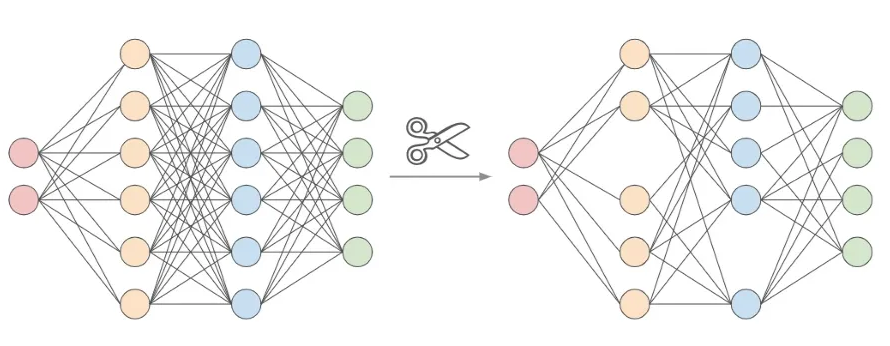
\includegraphics[scale=0.5]{03_capitulo/imagepruning.png}

\subsection{Passo a passo da Poda}
A poda tenta identificar e remover parâmetros desnecessários para criar um modelo menor e mais eficiente, sem sacrificar muito a precisão.
\begin{itemize}
    \item \textbf{Passo 1 (Definição de critérios e taxa de poda):} A partir de um modelo já treinado e denso, atribui a importância dos parâmetros da rede, os valores finais dos pesos, que indica quais conexões são cruciais e quais não são. Dessa forma define o critério de quais pesos são desnecessários, o mais comum é a poda por magnitude, onde os pesos com valores absolutos mais baixos são considerados menos importantes. Define também a taxa de esparsidade, que é a porcentagem de pesos que serão removidos.
    \item \textbf{Passo 2 (Identificação dos pesos a serem podados):} Com o critério e a taxa de poda definidos, o algoritmo inspeciona todos os pesos na rede e classifica-os com base em sua importância, selecionando os pesos que atendem ao critério de poda.
    \item \textbf{Passo 3 (Execução da poda):} Com todos os pesos classificados e os que serão podados selecionados, o algoritmo procede para remover esses pesos da rede, em que os pesos selecionados são definidos como zero, efetivamente removendo essas conexões da rede. Assim a rede fica esparsa, com a matriz de pesos contendo muitos zeros. Por se zerar muitos pesos, o modelo pode ser armazenado em formatos de matrizes esparsas, armazenando apenas os valores diferentes de zero e suas posições, tendo uma redução no tamanho do modelo.
    \item \textbf{Passo 4 (Ajuste fino com retreinamento):} Após a poda, o modelo perde precisão, então ocorre um ajuste fino, que é um retreinamento do modelo podado, onde o modelo é treinado novamente com os dados de treinamento, mas com uma taxa de aprendizado menor, para que os pesos restantes possam se reajustar e compensar as conexões que foram podadas, recuperando parte do desempenho perdido. Os pesos que foram zerados continuam zerados, o retreinamento é nos pesos que sobraram, adaptando e compensando os pesos removidos.
    \item \textbf{Passo 5 (Iteração):} A poda é feita de forma iterativa, podando e fazendo o ajuste fino, repetindo isso várias vezes, assim com a poda pouco a pouco a rede se adapta melhor às mudanças do que retirar uma taxa muito alta de uma vez, resultando em uma perda de acurácia menor.
\end{itemize}

\subsection{Utilização da Poda}
A grande maioria da utilização da poda, seja ela qual for, é feita após o treinamento do modelo, e que após isso é feito um ajuste fino para que o modelo se adapte à nova estrutura.
Contudo, métodos recentes realizam a poda de forma gradual durante o processo de treinamento, em que a cada uma quantidade de épocas estabelecida, podando o modelo aos poucos, assim a rede adapta-se à nova estrutura de forma mais eficiente.
Há um novo início de pesquisa em que busca podar uma rede neural antes do treinamento, em que tenta identificar sub-redes inerentemente boas, assim o treinamento é feito apenas nessas sub-redes, que já são menores e mais eficientes para o resultado final, isso faria com que economizasse ainda mais recursos computacionais, mas ainda é um campo em desenvolvimento impulsionado pela hipótese do Bilhete de Loteria (Lottery Ticket Hypothesis).

\section{Datasets}
Para a poda ser realizada, é necessário um conjunto de dados para que o modelo possa ser ajustado após a remoção dos pesos, assim o modelo consegue se adaptar à nova estrutura. Assim, foi selecionado o dataset ImageNet, que é um grande conjunto de dados de imagens rotuladas, amplamente utilizado para treinar e avaliar modelos de visão computacional, ele contém mais de 1,2 milhões de imagens de treinamento, dividido em 1000 classes diferentes, como animais, objetos, entre outros, sendo imagens do mundo real de alta resolução, com iluminação variadas, ângulos diferentes e fundos diversos, o que torna o dataset desafiador e realista.
O ImageNet é amplamente utilizado para tarefas de classificação de imagens, onde o objetivo é atribuir um rótulo correto a cada imagem com base em seu conteúdo visual. Ele também é usado para tarefas de detecção de objetos, onde o modelo deve identificar e localizar múltiplos objetos dentro de uma única imagem.
Para conseguir treinar a ImageNet, vieram modelos de redes neurais profundas e complexas que pudessem lidar com essa grande escala e dificuldade que o ImageNet apresenta.
Dessa forma, vieram diversos modelos famosos como VGG-16 e ResNet-50.
\subsection{VGG-16}
A VGG-16 é uma arquitetura de modelo de rede neural convolucional profunda desenvolvida pela Visual Geometry Group (VGG) da Universidade de Oxford, que ficou famosa por seu desempenho no ImageNet Large Scale Visual Recognition Challenge (ILSVRC) em 2014.
Sendo um modelo de 16 camadas, em que o modelo não cria blocos complexos, ela utiliza uma arquitetura de força bruta, muito profunda e uniforme, são pilhas de camadas de convolução 3x3 e camadas MaxPooling 2x2.
\subsection{ResNet-50}
A ResNet-50 é a arquitetura de rede neural convolucional profunda que faz parte da família ResNet (Redes Neurais Residuais), desenvolvida pela Microsoft Research, que também teve um desempenho notável no ImageNet Large Scale Visual Recognition Challenge (ILSVRC) em 2015.
A ResNet se diferencia por introduzir uma solução de conexão de atalho (skip connections), que permite que o gradiente flua diretamente através de várias camadas, mitigando o problema do desaparecimento do gradiente em redes muito profundas. Em outros casos, uma informação tinha de passar por todas as camadas e podia se perder essa informação devido ao alto número de camadas, na ResNet ele cria de certa forma, "atalhos" para que a informação possa pular algumas camadas e chegar mais rápido ao destino, assim o modelo consegue ser mais profundo sem perder a capacidade de aprendizado.
Utiliza blocos residuais, onde a entrada de um bloco é somada a sua saída, permitindo que o modelo aprenda a função residual, ou seja, a diferença entre a entrada e a saída desejada, ao invés de aprender a função completa, assim sua estrutura usa uma sequência de 3 camadas para economizar cálculos, sendo uma camada 1x1 convolucional para compressão, uma camada 3x3 convolucional para extração de características e uma camada 1x1 convolucional para expansão, sendo isso repetido diversas vezes, totalizando 50 camadas.
\section{Pytorch}
Pytorch é uma biblioteca de aprendizado de máquina de código aberto desenvolvida pelo Facebook's AI Research lab (FAIR), amplamente utilizada para tarefas de visão computacional e processamento de linguagem natural.
Ela fornece uma interface flexível e dinâmica para construir e treinar redes neurais, permitindo que os desenvolvedores criem modelos complexos de forma intuitiva.
Uma das principais características do Pytorch é seu sistema de computação automática de gradientes, que facilita o processo de backpropagation, permitindo que os desenvolvedores calculem automaticamente os gradientes necessários para otimizar os pesos da rede neural durante o treinamento, além de possuir uma aceleração de GPU via CUDA, que permite que os modelos sejam treinados de forma eficiente em hardware especializado, acelerando significativamente o processo de treinamento.
\section{Métricas de Avaliação}
\subsection{Acurácia}
Métrica de performance amplamente utilizada em tarefas de classificação, que mede a proporção de previsões corretas feitas pelo modelo em relação ao total de previsões realizadas, ou seja, a porcentagem de previsões que o modelo acertou em relação ao número total de amostras. No atual contexto, a acurácia é a principal métrica de performance, pois estamos tentando preservá-la ao máximo possível durante o processo de poda.
\subsection{Tempo de Inferência}
Tempo de relógio que o modelo leva para processar um conjunto de dados, através dela tem-se a medida prática da velocidade do modelo, a latência é crucial em aplicações em tempo real, onde respostas rápidas são essenciais, como em sistemas de recomendação, reconhecimento de voz e veículos autônomos. O tempo de inferência é medido utilizando a biblioteca \textit{time} do Python, que permite medir o tempo decorrido entre o início e o fim do processo de inferência, fornecendo uma métrica direta da eficiência do modelo.
\subsection{Consumo de energia}
Mede a quantidade de energia elétrica consumida pelo modelo durante todo o processo. Está sendo calculado pela biblioteca \textit{CodeCarbon}, que monitora o consumo de energia e as emissões de carbono associadas ao treinamento e à inferência de modelos de aprendizado de máquina. A biblioteca rastreia o uso de energia do hardware, como CPUs e GPUs, e estima as emissões de carbono com base na localização geográfica e na fonte de energia utilizada. O objetivo é fornecer insights sobre o impacto ambiental dos modelos de aprendizado de máquina.
